% !TEX root = /home/frank/School/thesis_text/thesis.tex

\chapter{Performance Analysis}

\section{Roofline Model}

The roofline model as proposed provides a visual model to gain insight into the factors influencing the performance of multicore CPU's.\cite{Williams:2009:RIV:1498765.1498785}
It is based on the observation that the off-chip memory bandwidth is the constraining resource on the performance of a system.\cite{patterson2004latency}  The roofline model is a plot of the attainable floating point operations per second in function of the computational intensity. The computational intensity (CI) is the number of floating-point operations per byte fetched from the off-chip RAM memory. The roofline model thus relates the demands of an application on the memory system to the maximum attainable performance.
An example plot of the roofline model is given in figure \ref{img:roofline_example}.\\

There are two main factors influencing the upper bound on the performance. The first one is the peak memory bandwidth (BW). The peak memory bandwidth is represented by the sloped black line on the left side of the graph in figure \ref{img:roofline_example}. An application that hits the roof in this area is called memory bound. An example of an computational intensity resulting in memory-bound operation is given by the red line in \ref{img:roofline_example} With increasing computational intensity the performance increases up to the ridge point. The x-coordinate of the ridge point represents the minimal computational intensity an application needs to reach to get maximum performance from the architecture. This maximum performance is the maximum computational performance (CP) and is represented by the flat line on the right side of figure \ref{img:roofline_example}. The dashed blue line shows an application of which the performance hits the roof in the computational performance area.
The relation between CI, BW and CP are given by the following formula.

\begin{equation}
Attainable\;GFlops/sec = min \left( BW \times CI \; , \; CP \right)
\end{equation}

The roofline model provides an upper bound to the performance of a certain architecture, but an application is not guaranteed to perform at this upper bound. Only if sufficient use is made of the available resources and optimizations, can the performance reach the roof. The effect on the maximum attainable performance on the performance of an architecture can be represented by what is called a \emph{ceiling}. In figure \ref{img:roofline_example} there are 2 examples of a ceiling: an I/O bandwidth ceiling represented by the dashed cyan line and a computational ceiling represented by the dashed green line. 

\begin{figure}[H]
\centering
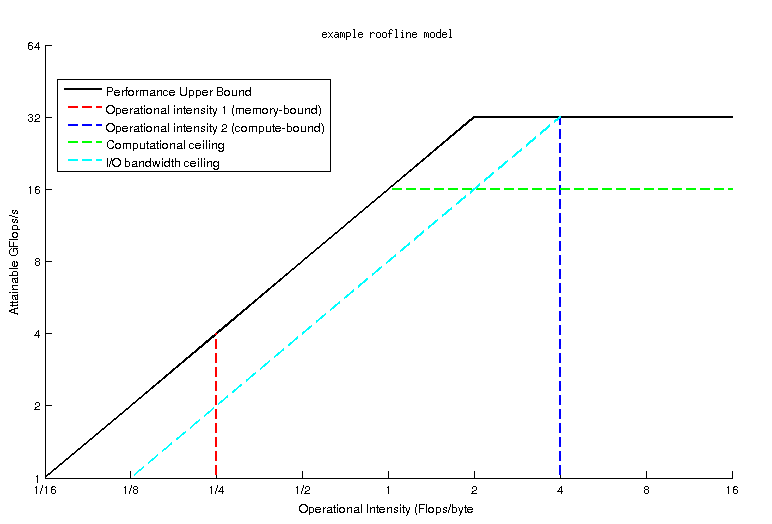
\includegraphics[scale=0.6]{./images/matlab_plots/roofline_example.png}
\caption{Example of a roofline model}
\label{img:roofline_example}
\end{figure}

Although the roofline model has been conceived as a tool for the estimation of performance of multicore CPU architectures, it has been adapted for use with other architectures such as GPU's\cite{spieringsembedded} and FPGA's\cite{spieringsembedded,daperformance}.
The roofline model in it's default form is inadequate to describe the maximum attainable performance of an FPGA based system because of the flexibility of FPGA's. In \cite{daperformance} a number of extensions are proposed to make the roofline model more suitable for FPGA's:
\begin{description}
	
	\item[Operations] Because floating-point operations are prohibitively expensive area-wise, they are often replaced by alternatives such as fixed-point operations. For this reason byte-operations [Bops] are proposed as a more general alternative to the more CPU/GPU specific floating-point operations.

	\item[Scalability] A processing element (PE) is defined as the hardware that contains all the necessary resources to perform the functionality of the algorithm. If the FPGA has enough resources this allows for multiple instantiations of the PE. The scalability factor is given by following formula:

	\begin{equation}
		SC = \left[\frac{Available\;Resources}{Resource\;consumption \; per \; PE}\right]
	\end{equation}

	The attainable performance of one PE needs to be multiplied by the scalability factor.

	\begin{equation}
		Attainable \; Performance = min(CP_{PE} \times SC, CI \times BW)
	\end{equation}

	This relates computational performance to resource consumption.

	\item[I/O bandwidth] In the original roofline model the off-chip memory is considered as the only bound on the performance of a system. Because of the nature of FPGA's where multiple means of I/O are available at the same time these all have to be considered. The roofline model should all take these into consideration and thus have an I/O bandwidth roof and possibly multiple I/O bandwidth ceilings.

	\item[Roofs and ceilings] Due to the fact that the computational intensity and the computational performance are both dependent on the implementation of the algorithm, the computational performance roofline will no longer be a constant. Also a number of ceilings have to be included to represent the different optimization and I/O possibilities.

	\item[Computational intensity] Because the CI influences both the SC and the CP$_{PE}$, it is the key to determining the roofline model. In the original roofline model the CI is modified through the use of code adjustments or optimizations. In the roofline model for FPGA the preferred methods of modifying the CI is through optimizations or through increasing the data locality of the implementation. An example of an optimization that influences the CI is loop unrolling.

\end{description}

\section{Factors influencing performance in a Vivado HLS core}

Video processing systems usually employ buffers to benefit from spatial and temporal locality of reference. In the example of the TRD there are 2 abstractions implemented: \texttt{ap\_linebuffer} and \texttt{ap\_window}.

\subsection{\texttt{ap\_linebuffer} Class}

The class \texttt{ap\_linebuffer} is a generic C++ implementation of the linebuffer described in XAPP793. A linebuffer is described as a multi-dimensional shift-register. A linebuffer needs to be able to be read and written to in the same cycle to maximize performance. The dual port nature of block RAM makes it the ideal component for this abstraction.
Because the \texttt{ap\_linebuffer} class is generic its behavior needs to be defined in the application. The template for the \texttt{ap\_linebuffer} class is \texttt{<typename T, int LROW, int LCOL>}. A type, the number of rows and the number of columns need to be specified. These definitions are in the \texttt{sobel.h} file:


\skipbig{\hlsdirective{typedef ap\_linebuffer<unsigned char, 3, MAX\_WIDTH> Y\_BUFFER;}}


The parameters of the template are used to determine the size of the only variable of the class, -the array M of type T with LROW rows and LCOL columns.\\
This array gets partitioned by the following directive:

\skipbig{\hlsdirective{\#pragma AP ARRAY\_PARTITION variable=M dim=1 complete}}


This means that the first dimension, the number of rows, get partitioned into different block RAMs. This is also reported by the Vivado HLS tool. buff\_A is the line buffer used throughout the implementation.\\

\medskip

\begin{figure}[h]
\centering
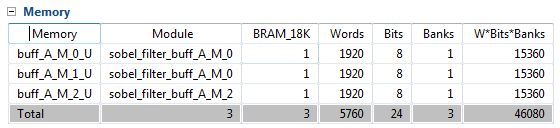
\includegraphics[scale=0.8]{/home/frank/School/thesis_text/images/trd_original_buffer_partitioning.PNG} 
\caption{Partitioning of an array in multiple block RAM instances}
\end{figure}


\subsection{\texttt{ap\_window} Class}

The second class used in the application is a generic implementation of the memory window described in XAPP793. It is a combination of shift-registers forming a 2-dimensional data storage element of N pixels centered on a pixel P. Usually these are implemented as flip-flops because they contain relatively few elements who need to be simultaneously available for a calculation. This is achieved through completely partitioning the memory into registers, preventing it from being implemented by a block RAM.
The template of \texttt{ap\_window} is \texttt{<typename T, int LROW, int LCOL>}. These parameters are used for the only variable in the class, an array M of type T with LROW rows and LCOL cols. Analog to the linebuffer class the programmer here also needs to define the type, number of rows and number of columns of array M. The array gets partitioned into registers by the following directive


\skipbig{\hlsdirective{\#pragma AP ARRAY\_PARTITION variable=M dim=0 complete}}


The \texttt{dim=0} means that all dimensions should be partitioned. The \texttt{complete} keyword signifies that this partitioning should be done for the whole array.


\subsection{Influence of memory architecture on the computational intensity}

This hierarchical structure of the memory influences the computational intensity of the algorithm. The numerator is determined by the number of bytes being processed by the core. Every iteration one value gets read from the external memory and one value gets written.  There are 32 bits per pixel, so there are 4 bytes per pixel. This means that with height H and width W there are:

\begin{equation} \label{eq:orig_den}
4 * 2 * ( H * W )
\end{equation}

bytes being read or written to or from the memory. This is the denominator in the expression of the computational intensity.\\
The numerator is dependent on the number of pixels being calculated by the core. The implementation of the Sobel core doesn't calculate the values on the pixels of the outer rim, as can be seen in code listing \ref{lst:sobelpix}

\begin{lstlisting}[caption=Sobel Code Snippet, captionpos=b, label=lst:sobelpix]

if( row <= 1 || col <= 1 || row > (rows-1) || col > (cols-1)){
		
		edge.R = edge.G = edge.B = 0;
		
}
//Sobel operation on the inner portion of the image
else{

		edge = sobel_operator( ... );
		
}

\end{lstlisting}

This however doesn't influence the computational intensity if one interprets a processing element as being all the necessary resources to perform the functionality of the algorithm. Even more so, these pixels also have to be read from memory and are already present in the denominator part of the expression.


\begin{equation} \label{eq:orig_num}
( H * W )
\end{equation}

\medskip
Combining Equations \ref{eq:orig_den} and \ref{eq:orig_num} gives us
\medskip

\begin{equation}
CI = \frac{H \times W}{4 \times 2 \times ( H \times W )}
\end{equation}




\section{Directives influencing throughput}

\subsection{Original Directives}
\label{sec:original_pragma}

The original TRD has 3 directives applied to it:

\begin{itemize}
\item \hlsdirective{set\_directive\_loop\_flatten -off \\ "sobel\_filter/sobel\_filter\_label0"}
\item \hlsdirective{set\_directive\_dependence -variable \&buff\_A -type inter \\ -dependent false "sobel\_filter/sobel\_filter\_label0"}
\item \hlsdirective{set\_directive\_pipeline -II 1 \\ "sobel\_filter/sobel\_filter\_label0"}
\end{itemize}

\paragraph{Throughput}
\label{sec:original_througput}
Given the analysis generated by Vivado HLS, presented in table \ref{tab:analysis_data}, it is possible to calculate the throughput of the system. First of all it needs to be noted whether the system satisfies the timing requirements. The analysis gives us an estimated clock period of 4.2 ns with an uncertainty of 0.62 ns placing it well within the bounds of the required 5 ns clock period.
The system needs 22 cycles to complete. Of these, there are 2 initialization cycles, 20 cycles to finish the outer loop, of which 19 cycles are the inner loop. The system employs pipelining on the innermost loop, which results in an initiation interval of 1.

I denotes a number of iterations, n a number of cycles. N is the number of cycles necessary to calculate one frame:

\begin{equation}\label{eq:nframes_orig_trd}
N_{frame} = n_{init} + I_{outer\;loop} \times ( n_{inner\;loop} + I_{inner\;loop} - 1 )
\end{equation}

% \[
% N =  \text{init cycles} + \text{outer loop iterations} * ( \text{iteration cycles} + \text{inner loop iterations} - 1)
% \]


These cycles all take one clock period to complete:

\begin{equation}\label{eq:frametime}
t_{frame} = N_{frame} * T_{clock}
\end{equation}

The number of frames per second is then given by:

\begin{equation}\label{eq:fps}
FPS = \frac{1}{t_{frame}}
\end{equation}

Entering the numbers found in table \ref{tab:analysis_data} gives us a value of 95.37 frames per second. Given that HDMI has a 60 Hz refresh rate this system satisfies that constraint.


\subsection{No directives}
\label{sec:nopragma}

The original system performance satisfies the real time constraint placed on the system. To study the impact the directives have on the performance of the system, all directives were removed from the  system. The analysis generated by Vivado HLS is presented in the second column of table \ref{tab:analysis_data}. The first observation that can be made is that the system performs the same operation in only 16 clock cycles instead of 22, a decrease of 27\%. Because the system has no pipelining, the initiation interval is 14 cycles. A new value gets read each iteration.

The number of cycles needed to calculate one frame is given by:

\begin{equation}
N = n_{init} + I_{outer\;loop} \times (I_{inner\;loop} \times n_{inner\;loop})
\end{equation}

% \[
% N = init\ cycles + outer\ loop\ iterations * (inner\ loop\ iterations * inner\ loop\ cycles) 
% \]


Knowing the number of cycles the throughput can be calculated using formulas \ref{eq:frametime} and \ref{eq:fps} and the information found in table \ref{tab:analysis_data} . This gives us a value of 0.47 frames per second, a 203 times decrease in performance.

\subsection{Other combinations of directives}

It is clear that these directives have a profound effect on the performance of a system. Also noteworthy is that the directives presented in section \ref{sec:original_pragma} in no way influence the computational intensity of the implementation. Each combination of these directives can thus be represented as a ceiling in the roofline model.
All sensible combinations of these directives have been tested and the results are represented in table  \ref{tab:analysis_data}. The corresponding resource utilization estimates are presented in table \ref{tab:utilization_estimates}.

\paragraph{Only Dependence}
Using only the following directive

\skipbig{\hlsdirective{set\_directive\_dependence -variable \&buff\_A -type inter \\ -dependent false "sobel\_filter/sobel\_filter\_label0"}}

doesn't have any measurable effect on the performance on the system compared to the one presented in section \ref{sec:nopragma}. The calculations for the performance stay the same at 0.47 FPS.

\paragraph{Only Loop Flattening}
Using only the following directive

\skipbig{\hlsdirective{set\_directive\_loop\_flatten "sobel\_filter/sobel\_filter\_label0"}}

combines the 2 loops iterating over the rows and the columns into 1 loop. Because this means that there is only one iteration to take into account, this changes the throughput of the system. The number of cycles necessary to process a frame is given by:

% 1/((init cycles + (outer loop iterations * inner loop iterations) * outer loop cycles)

\begin{equation}
N = n_{init} + (I_{outer\;loop} \times I_{inner\;loop}) \times n_{loop}
\end{equation}

\bigskip

Using formulas \ref{eq:frametime} and \ref{eq:fps} and the values found in \ref{tab:analysis_data}, a performance of 6,88 FPS can be calculated. 

\paragraph{Only pipelining} Using the following directive

\skipbig{\hlsdirective{set\_directive\_pipeline -II 1 "sobel\_filter/sobel\_filter\_label0"}}

Flattens the loops and pipelines them. This has a profound effect on the system performance. II is the initiation interval.

%((Init + outer loop cycles  + ((outer loop iterations * inner loop iterations)-1) * initiation interval)

\begin{equation} \label{eq:only_pipelining}
N  = n_{init} + n_{outer\;loop} + ((I_{inner\;loop} \times I_{outer\;loop}) - 1) \times II
\end{equation}

\bigskip

Using the values found in table \ref{tab:analysis_data} gives a performance of 48.15 FPS. This is a considerable improvement but doesn't reach the required 60 FPS to satisfy the requirements placed on the system by the HDMI protocol. Noteworthy in this case is that the system has an initiation interval of 2. This causes a pixel to be output only every 2 cycles instead of every cycle after the first iteration. The compiler defaults to the lowest II it can use. As an experiment the initiation interval was set to 2 in the directive. This didn't have any measurable influence on the system.

\paragraph{Loop flattening on}
Using following directives:

\begin{itemize}
\item \hlsdirective{set\_directive\_dependence -variable \&buff\_A -type inter \\ -dependent false "sobel\_filter/sobel\_filter\_label0"}
\item \hlsdirective{set\_directive\_pipeline -II 1  \\ "sobel\_filter/sobel\_filter\_label0"}
\item \hlsdirective{set\_directive\_loop\_flatten  \\ "sobel\_filter/sobel\_filter\_label0"}
\end{itemize}

This flattens the loops, pipelines them and takes into consideration that there is no inter-iteration dependence conflict for the buff\_A. The expression for the number of cycles necessary is the same as in equation \ref{eq:only_pipelining}. The most notable difference is that the initiation interval is equal to 1. This gives a performance of 91.72 FPS. Vivado HLS predicts in it's synthesis report that the system will have a minimum clock period 5.25 ns. This leaves the risk that the core will cause glitches and not satisfy the requirements. Increasing the II to 2 makes the system respect the timing constraints again but lowers the performance to 48.15 FPS. 

\paragraph{No dependence}
Using following directives:

\begin{itemize}
\item \hlsdirective{set\_directive\_loop\_flatten -false  \\ "sobel\_filter/sobel\_filter\_label0"}
\item \hlsdirective{set\_directive\_pipeline -II 1  \\ "sobel\_filter/sobel\_filter\_label0"}
\end{itemize}

The only difference with the directives of the original TRD is that the compiler isn't notified of the fact that there is no inter-dependence for the \texttt{buff\_A} variable. The same equation for the performance is given by eq. \ref{eq:nframes_orig_trd}. Using the values found in table \ref{tab:analysis_data} a performance of 95.31 FPS cam be calculated, only marginally worse than the performance of the original configuration. 


\section{Resource consumption}

The resource consumption estimates for these different solutions are given in table \ref{tab:utilization_estimates}. The utilization estimates are of importance because they determine the scalability of a core and thus the maximum attainable performance. Of all the combinations of directives that were tested only the original configuration and the no\_dependence configuration satisfied the requirements for the system. Given that the resource consumption is identical for the original configuration and the no\_dependence configuration the only determining factor in choosing is the performance. Given that the original configuration has better performance, although marginally, it is the most sensible choice to use for the building of a roofline model.\\



% Table specifying the resource consumption of the different solutions

\begin{table}[H]
\begin{center}
\begin{tabular}{rcccc}
\toprule
 & \textbf{BRAM\_18K} & \textbf{DSP48E} & \textbf{FF} & \textbf{LUT}\\ \midrule
\textbf{Original directives} & 3 & 23 & 1487 & 1412 \\ 
\textbf{No pragma} & 5 & 4 & 802 & 1475 \\ 
\textbf{loop\_flatten\_on} & 3 & 23 & 1764 & 1668 \\ 
\textbf{loop\_flatten\_II\_2} & 3 & 23 & 1777 & 1875 \\ 
\textbf{no\_dependence} & 3 & 19 & 1487 & 1412 \\ 
\textbf{no\_pipeline} & 5 & 4 & 802 & 1475 \\ 
\textbf{only dependence} & 5 & 4 & 786 & 1534 \\ 
\textbf{only loop flattening} & 5 & 8 & 1050 & 1783 \\ 
\textbf{only pipelining} & 3 & 23 & 1851 & 1849 \\ \bottomrule
\end{tabular}
\end{center}
\caption{Utilization Estimates}
\label{tab:utilization_estimates}
\end{table}




The original solution was exported as a Xilinx PCore and connected to the TRD system. This system was synthesized to get a more accurate prediction of the resource consumption. The results are detailed in table \ref{tab:scalability}. The difference between the roofline model of the The first noticeable difference when comparing the HLS estimates to the utilization reported from PlanAhead, found on the FILTER\_ENGINE line of the table, is that only the number of reported DSP blocks remains the same. The differences between the other reported values are likely caused by the addition of the AXI wrapper and possible redundancies in the design. The system also uses a number of IP-cores to perform necessary transformations on the data. They do not need to be duplicated to scale the system so these resources can be considered an overhead. Only the filter engine and the associated DMA engine need to be duplicated.\\
The resource consumption in the Zynq differs from the resource consumption for regular FPGA's in that the available interfaces also need to be considered. The Zynq has 4 AXI High Performance ports and these are the constraining factor on the scalability of the TRD core. The filter engine/VDMA combination can be duplicated 3 times. 

% !TEX root = /home/frank/School/thesis_text/thesis.tex


% \begin{table}[H]
% \begin{center}
% \begin{tabular}{rcccc}
% \toprule
%  & \textbf{Register} & \textbf{LUT} & \textbf{BRAM} & \textbf{DSP48} \\ \midrule 
% \textbf{Total n$^{\circ}$ available} & 319200 & 159600 & 140 & 220 \\ 
% \textbf{Total Used} & 27648 & 25804 & 30 & 39 \\ 
% \textbf{FILTER\_ENGINE} & 1965 & 2156 & 2 & 23 \\ 
% \textbf{Overhead} & 25683 & 23648 & 28 & 16 \\ 
% \textbf{Max  available resources} & 293517 & 135952 & 112 & 204 \\ 
% \textbf{Max possible instances} & 149,37 & 63,057 & 56 & 8,87 \\ 
% \textbf{Rounded} & 149 & 63 & 56 & 8 \\ \bottomrule
% \end{tabular}
% \caption{Scalability of the TRD}
% \label{tab:scalability}
% \end{center}
% \end{table}

% \begin{table}[H]
% \begin{center}
% \begin{tabular}{rcccc}
% \toprule
%  & \textbf{Register} & \textbf{LUT} & \textbf{BRAM} & \textbf{DSP48} \\ \midrule 
% \textbf{Total n° available} & 319200 & 159600 & 140 & 220 \\ 
% \textbf{Total Used} & 27648 & 25804 & 30 & 39 \\ 
% \textbf{FILTER\_ENGINE} & 1965 & 2156 & 2 & 23 \\ 
% \textbf{FILTER\_VDMA} & 4176 & 3883 & 6 & 0 \\ 
% \textbf{Overhead} & 21507 & 19765 & 22 & 16 \\ 
% \textbf{Max  available resources} & 297693 & 139835 & 118 & 204 \\ 
% \textbf{Max possible instances} & 48,48 & 23,16 & 14,75 & 8,87 \\ 
% \textbf{Rounded} & 48 & 23 & 14 & 8 \\ \bottomrule
% \end{tabular}
% \caption{Scalability of the TRD}
% \label{tab:scalability}
% \end{center}
% \end{table}

\begin{table}[H]
\begin{center}
\scalebox{0.75}{
\begin{tabular}{rccccc}
\toprule
 									& \textbf{Register} 		& 	\textbf{LUT}		& 	\textbf{BRAM} 		& 	\textbf{DSP48} 		& \textbf{AXI HP} 	\\ \midrule
\textbf{n$^{\circ}$ available} 		& 		319200 				& 		159600 			& 		140 			& 		220 			& 	4 				\\ \medskip
\textbf{System consumption} 		& 		27648 (8.6\%) 		& 		25804 (16.2\%)	& 		30 (21.4\%)		& 		39 (17.7\%) 	& 	2 (50\%) 		\\ 
\textbf{FILTER\_ENGINE} 			& 		1965 (0.6\%)		& 		2156 (1.4\%)	& 		2 (1.4\%)		& 		23 (10.5\%)		& 	0 				\\ \medskip  
\textbf{FILTER\_VDMA} 				& 		4176 (1.3\%)		& 		3883 (2.4\%)	& 		6 (4.3\%)		& 		0 				& 	1 (25\%)		\\ 
\textbf{Overhead} 					& 		21507 (6.7\%)		& 		19765 (12.4\%)	& 		22 (15.7\%)		& 		16 (7.3\%)		& 	1 (25\%)		\\ 
\textbf{Max  available resources} 	& 		297693 (93.3\%)		& 		139835 (87.6\%)	& 		118 (84.3\%)	& 		204 (92.7\%)	& 	3 (75\%)		\\ \midrule
%\textbf{Max possible instances} & 48,48 & 23,16 & 14,75 & 8,87 & 3 \\ 
\textbf{Max Instances} 				& 		48 					& 		23 				& 		14 				& 		8 				& 	3 \\ \bottomrule
\end{tabular}
}
\caption{Scalability of the TRD}
\label{tab:scalability}
\end{center}
\end{table}

\section{Memory Bandwidth}

The memory bandwidth is the decisive factor in determining the performance of a system. In the case of the Zynq however the PS and PL are connected to the AXI interconnect switches. The different AXI interconnect possibilities all influence the maximum attainable memory bandwidth, as well as the DMA controllers utilizing these interconnects. The DDR memory has a bus width of 32 bits and a clock frequency of 1066MHz Providing a maximum bandwidth of 4264 MB/s \cite{anon._zynq-7000_2013}. The filter engine utilizes an AXI HP interconnect port, which in combination with a DMA controller have an estimates throughput of 1200 MB/s. The datasheet for the AXI VDMA controller v5.04a which is used in the system has similar figures, with a typical throughput of 539 MB/s for the MM2S channel and 542 MB/s throughput for the S2MM channel. These can be used in full-duplex which gives a total bandwidth of 1081 MB/s per AXI HP port\cite{axivdma}.
As the scalability has shown the AXI HP interfaces are the constraining factor on the performance of the system. In the case of the TRD only 3 interfaces can be used. This causes the maximum bandwidth to be $3 \times 1081$MB/s or 3243 MB/s. If all 4 interfaces would be used the DDR bandwidth would be the constraining factor. 

\section{Roofline Model}



\newpage
\begin{landscape}

\begin{table}[htbp]
\begin{center}

	\begin{tabular}{rccccc}
	\toprule
	 & \textbf{Original directives} & \textbf{No pragma} & \textbf{loop\_flatten\_on} & \textbf{loop\_flatten\_II\_2} & \textbf{no\_dependence} \\ \midrule
	
	\textbf{Estimated Clock (ns)} & 4,2 & 4,35 & 5,25 & 4,2 & 4,2 \\ 
	\textbf{Uncertainty (ns)} & 0,62 & 0,62 & 0,62 & 0,62 & 0,62 \\ 
	\textbf{cycle time (ns)} & 5 & 5 & 5,25 & 5 & 5 \\ 
	\textbf{total cycles} & 22 & 16 & 28 & 29 & 23 \\ 
	\textbf{init} & 2 & 2 & 8 & 8 & 2 \\ 
	\textbf{outer loop} & 20 & 14 & 20 & 21 & 21 \\ 
	\textbf{inner loop} & 19 & 13 & N/A & N/A & 20 \\ 
	\textbf{pipelining outer} & no & no & yes & yes & no \\ 
	\textbf{pipelining inner} & yes & no & N/A & N/A & yes \\ 
	\textbf{Initiation Interval} & 1 & 14 & 1 & 2 & 1 \\ \bottomrule
	\end{tabular}

	\bigskip

	\begin{tabular}{rccccc}
	\toprule
	 & \textbf{no\_pipeline} & \textbf{only dependence} & \textbf{only loop flattening} & \textbf{only pipelining} & \textbf{only pipelining II 2} \\ \midrule
	\textbf{Estimated Clock (ns)} & 4,35 & 4,35 & 4,35 & 4,2 & 4,2 \\ 
	\textbf{Uncertainty (ns)} & 0,62 & 0,62 & 0,62 & 0,62 & 0,62 \\ 
	\textbf{cycle time (ns)} & 5 & 5 & 5 & 5 & 5 \\ 
	\textbf{total cycles} & 17 & 16 & 22 & 31 & 31 \\ 
	\textbf{init} & 2 & 2 & 8 & 8 & 8 \\ 
	\textbf{outer loop} & 15 & 14 & 14 & 23 & 23 \\ 
	\textbf{inner loop} & 14 & 13 & N/A & N/A & N/A \\ 
	\textbf{pipelining outer} & no & no & no & yes & yes \\ 
	\textbf{pipelining inner} & no & no & no & no & no \\ 
	\textbf{Initiation Interval} & 15 & 14 & 14 & 2 & 2 \\ \bottomrule
	\end{tabular}


\end{center}
\caption{Analysis Data}
\label{tab:analysis_data}
\end{table}
\end{landscape}

% \begin{landscape}
% \begin{table}[htbp]
% \begin{center}
% \begin{tabular}{|r|r|r|r|r|r|}
% \hline
%  & \textbf{no\_pipeline} & \textbf{only dependence} & \textbf{only loop flattening} & \textbf{only pipelining} & \textbf{only pipelining II 2} \\ \hline
%  &  &  &  &  &  \\ \hline
% \textbf{Estimated Clock (ns)} & 4,35 & 4,35 & 4,35 & 4,2 & 4,2 \\ \hline
% \textbf{Uncertainty (ns)} & 0,62 & 0,62 & 0,62 & 0,62 & 0,62 \\ \hline
% \textbf{cycle time (ns)} & 5 & 5 & 5 & 5 & 5 \\ \hline
% \textbf{total cycles} & 17 & 16 & 22 & 31 & 31 \\ \hline
% \textbf{init} & 2 & 2 & 8 & 8 & 8 \\ \hline
% \textbf{outer loop} & 15 & 14 & 14 & 23 & 23 \\ \hline
% \textbf{inner loop} & 14 & 13 & N/A & N/A & N/A \\ \hline
% \textbf{pipelining outer} & no & no & no & yes & yes \\ \hline
% \textbf{pipelining inner} & no & no & no & no & no \\ \hline
% \textbf{Initiation Interval} & 15 & 14 & 14 & 2 & 2 \\ \hline
% \end{tabular}
% \end{center}
% \caption{Analysis Data Continued}
% \label{tab:analysis_data_cont}
% \end{table}
% \end{landscape}



